\documentclass[conference]{IEEEtran}
\usepackage{graphicx}
\usepackage{booktabs}
\usepackage{multirow}
\usepackage{amsmath,amssymb}
\usepackage{newtxtext,newtxmath}
\usepackage{xcolor}
\usepackage{url}
\usepackage{microtype}
\usepackage{balance}

\title{DASP-Park: Decision-Aware Active Semantic Perception for Reliable Parking-Slot Occupancy under Occlusion}

\author{\IEEEauthorblockN{Anonymous Author(s)}
\IEEEauthorblockA{Author information withheld for manuscript preparation}}

\begin{document}
\maketitle

\begin{abstract}
Reliable parking-slot selection is not equivalent to detecting an empty polygon in a single image or point cloud. In real parking scenes, mapped bays are observed from changing viewpoints, LiDAR returns from pillars and walls can resemble vehicles, camera projections can cross foreground objects, and many bays are genuinely unobservable. We present \emph{DASP-Park}, a decision-aware active semantic perception system that treats uncertainty as a first-class output. A causal geometric stage aggregates map-aligned LiDAR history and assigns each mapped bay one of \textsc{Free}, \textsc{Occupied}, or \textsc{Unknown}. Only unresolved bays in the forward $180^{\circ}$ driving region enter a bounded Plan--Execute--Observe agent. The agent autonomously selects camera context, image crop, or target-local LiDAR tools, while a deterministic validator binds every terminal decision to observed evidence and rejects unsupported model outputs. On a locked human annotation set at frame 6241 (14 bays: 6 Free, 2 Occupied, and 6 Unknown), the geometric stage attains 50.0\% three-class accuracy with 7.14\% terminal coverage. The complete camera-first system reaches 92.86\% accuracy and 64.29\% coverage, with all eight determinate bays classified correctly and one conservative-safety violation on an Unknown bay. A 16-setting temporal ablation selects $W{=}45,K{=}3$ under a safety-first criterion. A controlled local-VLM ablation further shows that capacity affects agent protocol adherence before visual accuracy: Qwen3-VL-2B invokes camera context for all 11 agent cases, whereas Qwen3.5-0.8B never enters the tool loop. Both ultimately fall back to Unknown under the unchanged safety contract. These results support a central design principle: in safety-relevant parking perception, an agent should choose evidence autonomously, but it should not be allowed to manufacture certainty.
\end{abstract}

\section{Introduction}
Autonomous parking requires a vehicle to reason about a deceptively difficult question: which mapped parking bay is both reachable and actually free? A nominal slot polygon may be behind the vehicle, outside the camera, hidden by a foreground vehicle, or intersected by returns from a pillar or wall. Conversely, a lack of LiDAR points inside a polygon does not prove free space unless sensor rays demonstrably traversed the target volume. These ambiguities are amplified in tight parking lots, where localization error is comparable to the clearance between adjacent bays.

Most parking perception systems are optimized to return a detection or occupancy label. This formulation encourages forced decisions in precisely those cases where observation is weakest. We instead formulate parking-slot occupancy as \emph{selective multimodal inference}: the system should emit a terminal label only when the available evidence supports it, and should preserve \textsc{Unknown} otherwise. The problem is therefore not only semantic classification, but also evidence acquisition, target ownership, and safe abstention.

DASP-Park separates these responsibilities. Part 1 is a deterministic, causal geometric triage stage. It aligns historical LiDAR observations in the map frame, evaluates target-interior free-space coverage and vehicle-like obstacle ownership, suppresses static structures, and retains explicit reason codes when evidence is insufficient. Part 2 is a bounded visual agent that receives the unresolved reasons and an environment-provided set of legal tools. A field-of-view check controls whether camera tools are available but does not inspect pixels or predict occupancy. The center model then plans which evidence to request, observes the structured tool return, and proposes a final three-state decision. A separate validator enforces evidence identity, modality-specific conditions, and a terminal confidence threshold.

Figure~\ref{fig:architecture} summarizes the resulting architecture. Unlike a fixed sensor-fusion pipeline, the center model chooses its next observation. Unlike an unconstrained vision-language model (VLM), however, it cannot bypass tool availability or cite evidence that was not observed. This division preserves agent autonomy while keeping safety-critical state transitions auditable.

This paper makes three contributions. First, we introduce a causal, map-aligned parking-slot formulation that represents Free, Occupied, and Unknown as distinct semantic outcomes and explicitly rejects pillar, wall, and boundary contamination. Second, we develop a camera-first Plan--Execute--Observe agent whose tools are selected autonomously but whose terminal states are accepted only under deterministic evidence contracts. Third, we provide a locked-GT evaluation with temporal and VLM-capacity ablations. The experiments expose both the benefit of agentic visual reasoning and a failure mode that aggregate accuracy alone would hide: small VLMs can return well-formed labels without ever acquiring the required visual evidence.

\begin{figure*}[t]
  \centering
  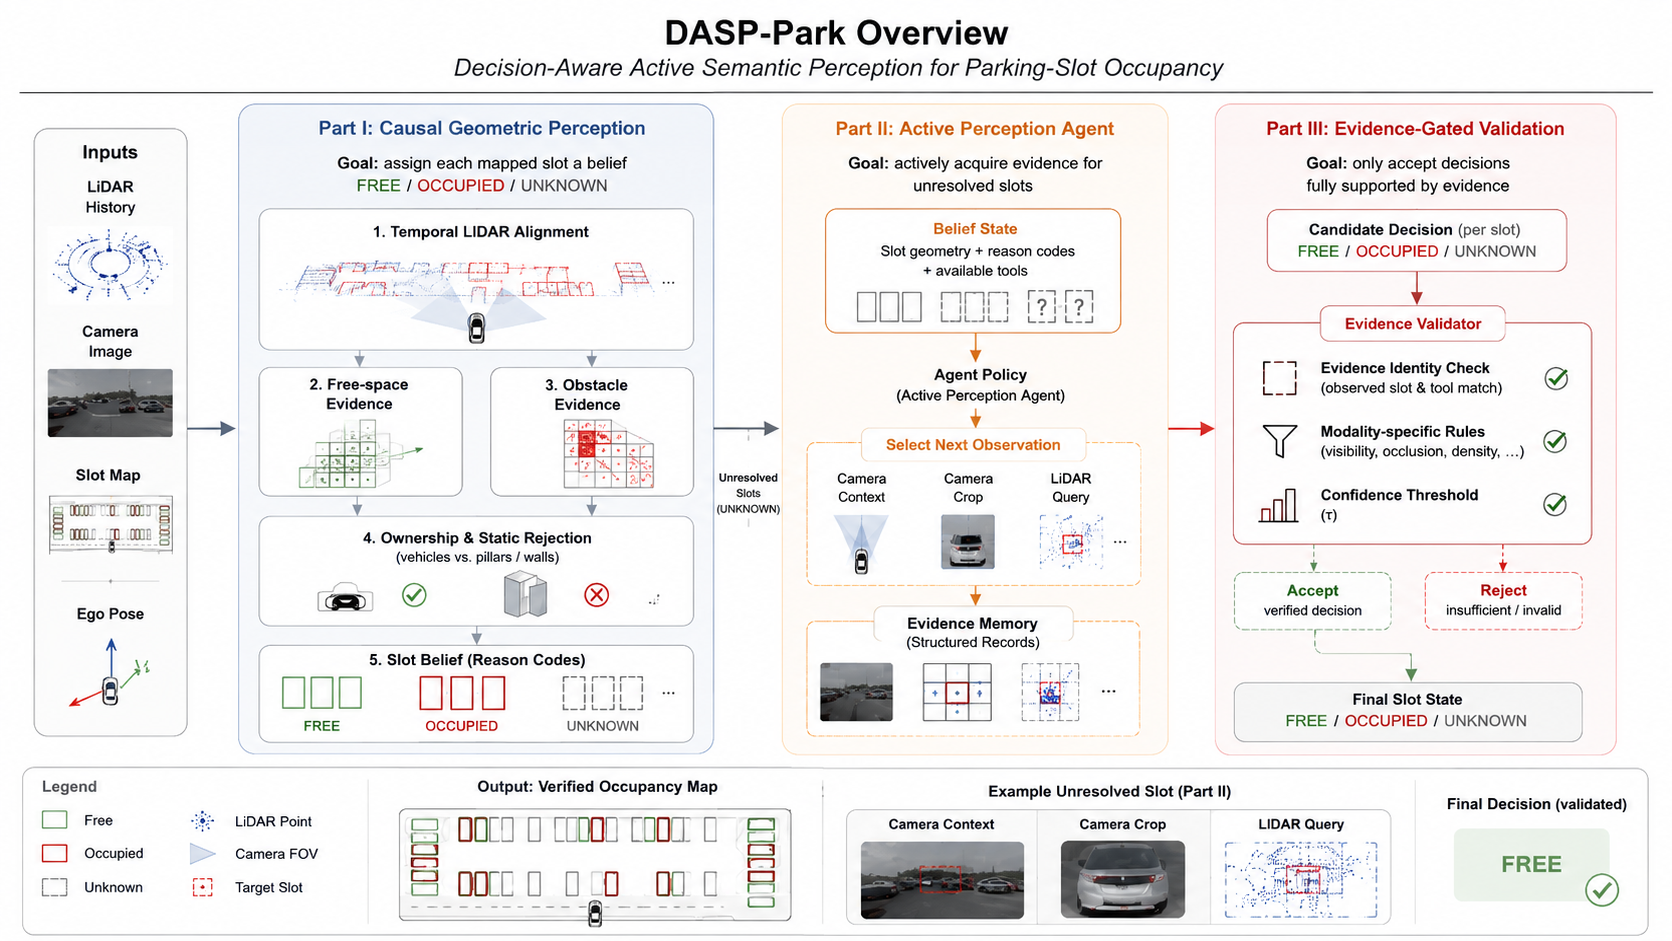
\includegraphics[width=0.99\textwidth]{figures/fig1_dasp_park_overview.png}
  \caption{DASP-Park system architecture. Causal map-aligned geometry separates terminal Free/Occupied evidence from unresolved Unknown cases. Only forward unresolved slots enter the camera-feasibility gate and the active-perception agent; an independent evidence validator controls final commitment.}
  \label{fig:architecture}
\end{figure*}

\section{Related Work}
\subsection{Parking-Slot Perception}
Classical parking-slot systems recover painted markings and their topology from surround-view imagery or geometric primitives~\cite{suhr2013parking,zinelli2019deep}. Learning-based detectors improve robustness to marking style, illumination, and perspective, but a detected slot boundary does not by itself establish current occupancy. Autonomous valet-parking systems additionally require metric localization and persistent maps~\cite{avpslam2020}. DASP-Park assumes a mapped slot inventory and focuses on a complementary problem: evidence-grounded occupancy of a known polygon under partial observation.

\subsection{Temporal 3D Perception and Sensor Fusion}
Modern 3D perception represents obstacles using point-based, pillar-based, or bird's-eye-view models~\cite{pointpillars2019,centerpoint2021}. Multi-sensor systems such as BEVFusion combine camera semantics with LiDAR geometry in a common representation~\cite{bevfusion2022}. These methods are powerful when trained with large-scale annotations, but their closed-set predictions do not directly encode whether a particular mapped bay was traversed by free-space rays or whether its returns belong to an adjacent object. Our approach uses temporal geometry as explicit evidence rather than treating absence of points as absence of an obstacle.

Registration quality is central to temporal aggregation. Iterative closest point and normal-distributions transform are standard foundations for aligning 3D observations~\cite{icp1992,ndt2003}. DASP-Park consumes corrected vehicle poses and retains conservative ownership margins and pose-perturbation checks. The aim is not a new localization algorithm; it is to prevent localization uncertainty from becoming false occupancy certainty.

\subsection{Agentic Visual Reasoning and Selective Prediction}
ReAct interleaves language-model reasoning with environment actions~\cite{react2023}, while Toolformer demonstrates that models can learn when to invoke external tools~\cite{toolformer2023}. Vision-language models such as Qwen3-VL extend this interaction to images, spatial content, and agentic decisions~\cite{qwen3vl2025}. DASP-Park adopts the action-observation abstraction but narrows it to a safety-bounded, single-slot decision. Tool output is structured, each evidence record is identity-bound, and unsupported final actions are rejected by runtime policy.

Selective classification studies the trade-off between coverage and correctness when a predictor may abstain~\cite{geifman2017selective}. Calibration and uncertainty estimation further caution that model confidence is not equivalent to empirical correctness~\cite{guo2017calibration,kendall2017uncertainty}. Our Unknown state combines semantic ambiguity, occlusion, missing observations, and contract failures. Accordingly, we report three-class accuracy, terminal coverage, selective accuracy, and false resolution of Unknown rather than a single accuracy number.

\begin{table}[t]
\centering
\caption{Positioning relative to representative system families.}
\label{tab:related}
\footnotesize
\resizebox{\columnwidth}{!}{%
\begin{tabular}{lcccc}
\toprule
Family & Map slot & Temporal 3D & Active tools & Explicit abstain \\
\midrule
Marking detector~\cite{suhr2013parking,zinelli2019deep} & -- & -- & -- & -- \\
BEV sensor fusion~\cite{bevfusion2022} & -- & \checkmark & -- & optional \\
General VLM agent~\cite{react2023,qwen3vl2025} & optional & optional & \checkmark & optional \\
DASP-Park & \checkmark & \checkmark & \checkmark & \checkmark \\
\bottomrule
\end{tabular}
}
\end{table}

\section{Methodology}
\subsection{Problem Formulation}
Let $\mathcal{S}=\{S_i\}$ be mapped parking-slot polygons and let $t_0$ denote the decision time. For each slot, the system estimates
\begin{equation}
 y_i \in \{\mathrm{Free},\mathrm{Occupied},\mathrm{Unknown}\}.
\end{equation}
The input comprises a causal LiDAR history, synchronized left-camera images, corrected poses, and the slot map. Ground-truth labels are never part of the inference request. The design objective is not maximum terminal coverage alone. We prioritize avoidance of unsupported Free or Occupied decisions and then resolve as many remaining cases as the evidence permits.

\subsection{Causal Map-Aligned Evidence}
Given a history span $W$ and sample count $K$, the causal sample set is
\begin{equation}
\begin{aligned}
j_m &= \operatorname{round}\!\left(\frac{m(W-1)}{K-1}\right),
      &&m=0,\ldots,K-1,\\
\mathcal{H}_{t_0}(W,K) &=
\left\{\mathcal{P}_{t_0}^{W}[j_m]\right\}_{m=0}^{K-1},
      &&K\geq2.
\end{aligned}
\end{equation}
where $\mathcal{P}_{t_0}^{W}$ is the ordered causal pool of the latest $W$ records. Rounding uniformly spaced pool indices reproduces the implemented sampler (for $W45/K3$: frames 6197, 6219, and 6241), always includes $t_0$, and never uses future observations. Each return $\mathbf{p}_{t}$ is transformed into the common map frame with the corrected pose $\mathbf{T}^{map}_{t}$.

For slot $S_i$, Part 1 constructs two complementary evidence families. Free-space evidence is accumulated only when measured LiDAR rays traverse the target volume; it includes volumetric coverage, near-ground coverage, viewpoint count, and angular separation. Obstacle evidence uses target-core support, vertical extent, temporal persistence, and vehicle-scale geometry. Static-structure and ownership vetoes suppress compact pillars, wall-like surfaces, boundary-dominated clusters, adjacent-slot overlap, and pose-sensitive hypotheses.

The Part 1 decision is expressed abstractly as
\begin{equation}
 \hat y_i^{(1)}=
 \begin{cases}
 \mathrm{Free}, & G_i^F=1 \land G_i^O=0,\\
 \mathrm{Occupied}, & G_i^O=1 \land G_i^F=0,\\
 \mathrm{Unknown}, & \text{otherwise},
 \end{cases}
\end{equation}
where $G_i^F$ combines positive ray-traversal and coverage tests, whereas $G_i^O$ combines target-owned obstacle support with the static-structure and pose-stability vetoes. Requiring mutual exclusion prevents conflicting evidence from becoming a terminal state. Unknown therefore has an explicit cause, such as occlusion, inadequate viewpoint separation, weak vehicle ownership, or static-boundary contamination; these reason codes are passed downstream.

\subsection{Forward Candidate Contract}
The system does not search behind the vehicle for a future parking action. An unresolved slot enters Part 2 only if
\begin{equation}
\begin{aligned}
q_i={}&\mathbb{1}[\hat y_i^{(1)}=\mathrm{Unknown}]\,
       \mathbb{1}[d_i\leq r]\\
     &\times\mathbb{1}\!\left[
       |\operatorname{wrap}(\psi_i-\psi_{\mathrm{ego}})|\leq\pi/2
       \right].
\end{aligned}
\end{equation}
where $d_i$ is distance to the ego pose, $r=18$~m, and the wrapped heading difference implements the forward $180^{\circ}$ half-plane. Camera feasibility is intentionally absent from this geometric candidate equation: \texttt{check\_fov} subsequently derives the legal tool set. This separation prevents a model from expanding its own search region or confusing sensor availability with occupancy.

\subsection{Camera-First Plan--Execute--Observe Agent}
Before the VLM is queried, \texttt{check\_fov} projects robust samples from the slot polygon using camera calibration. It returns visibility and legal tool names but does not inspect image content or classify occupancy. For camera-eligible cases, \texttt{camera\_context} is the mandatory first evidence tool. The returned causal contact sheet overlays the mapped target footprint in cyan. The VLM may then terminate, request a target crop, or invoke target-local LiDAR when target ownership is occluded or a projected vehicle may be foreground or adjacent.

At turn $k$, the center model receives belief state $b_k$, which contains the Part 1 reason, legal tools, and all observed evidence. Active perception is the recurrent process
\begin{equation}
\begin{aligned}
a_k &\sim \pi_{\theta}(\cdot\mid b_k,\mathcal{T}_k),\\
e_{k+1} &= \operatorname{Tool}(a_k),\\
b_{k+1} &= \mathcal{U}(b_k,e_{k+1}).
\end{aligned}
\end{equation}
where $\mathcal{T}_k$ is the environment-provided legal tool set, $e_{k+1}$ is a structured EvidenceRecord, and $\mathcal{U}$ updates the observable belief state. The policy may instead propose $\mathrm{Final}(\hat y_i)$. The action rationale is stored as a concise, auditable plan; hidden chain-of-thought is neither requested nor required. The loop is bounded to six model turns.

Figure~\ref{fig:active-agent} expands one audited OpenAI reference trajectory. The same center VLM first requests Camera context, observes a possible target/foreground ownership ambiguity, and autonomously requests target-local LiDAR. Because the LiDAR evidence remains non-terminal, validator feedback triggers a bounded Camera self-check before the final Occupied proposal is accepted. All arrows correspond to persisted structured actions or observations rather than a post-hoc workflow.

\begin{figure*}[t]
  \centering
  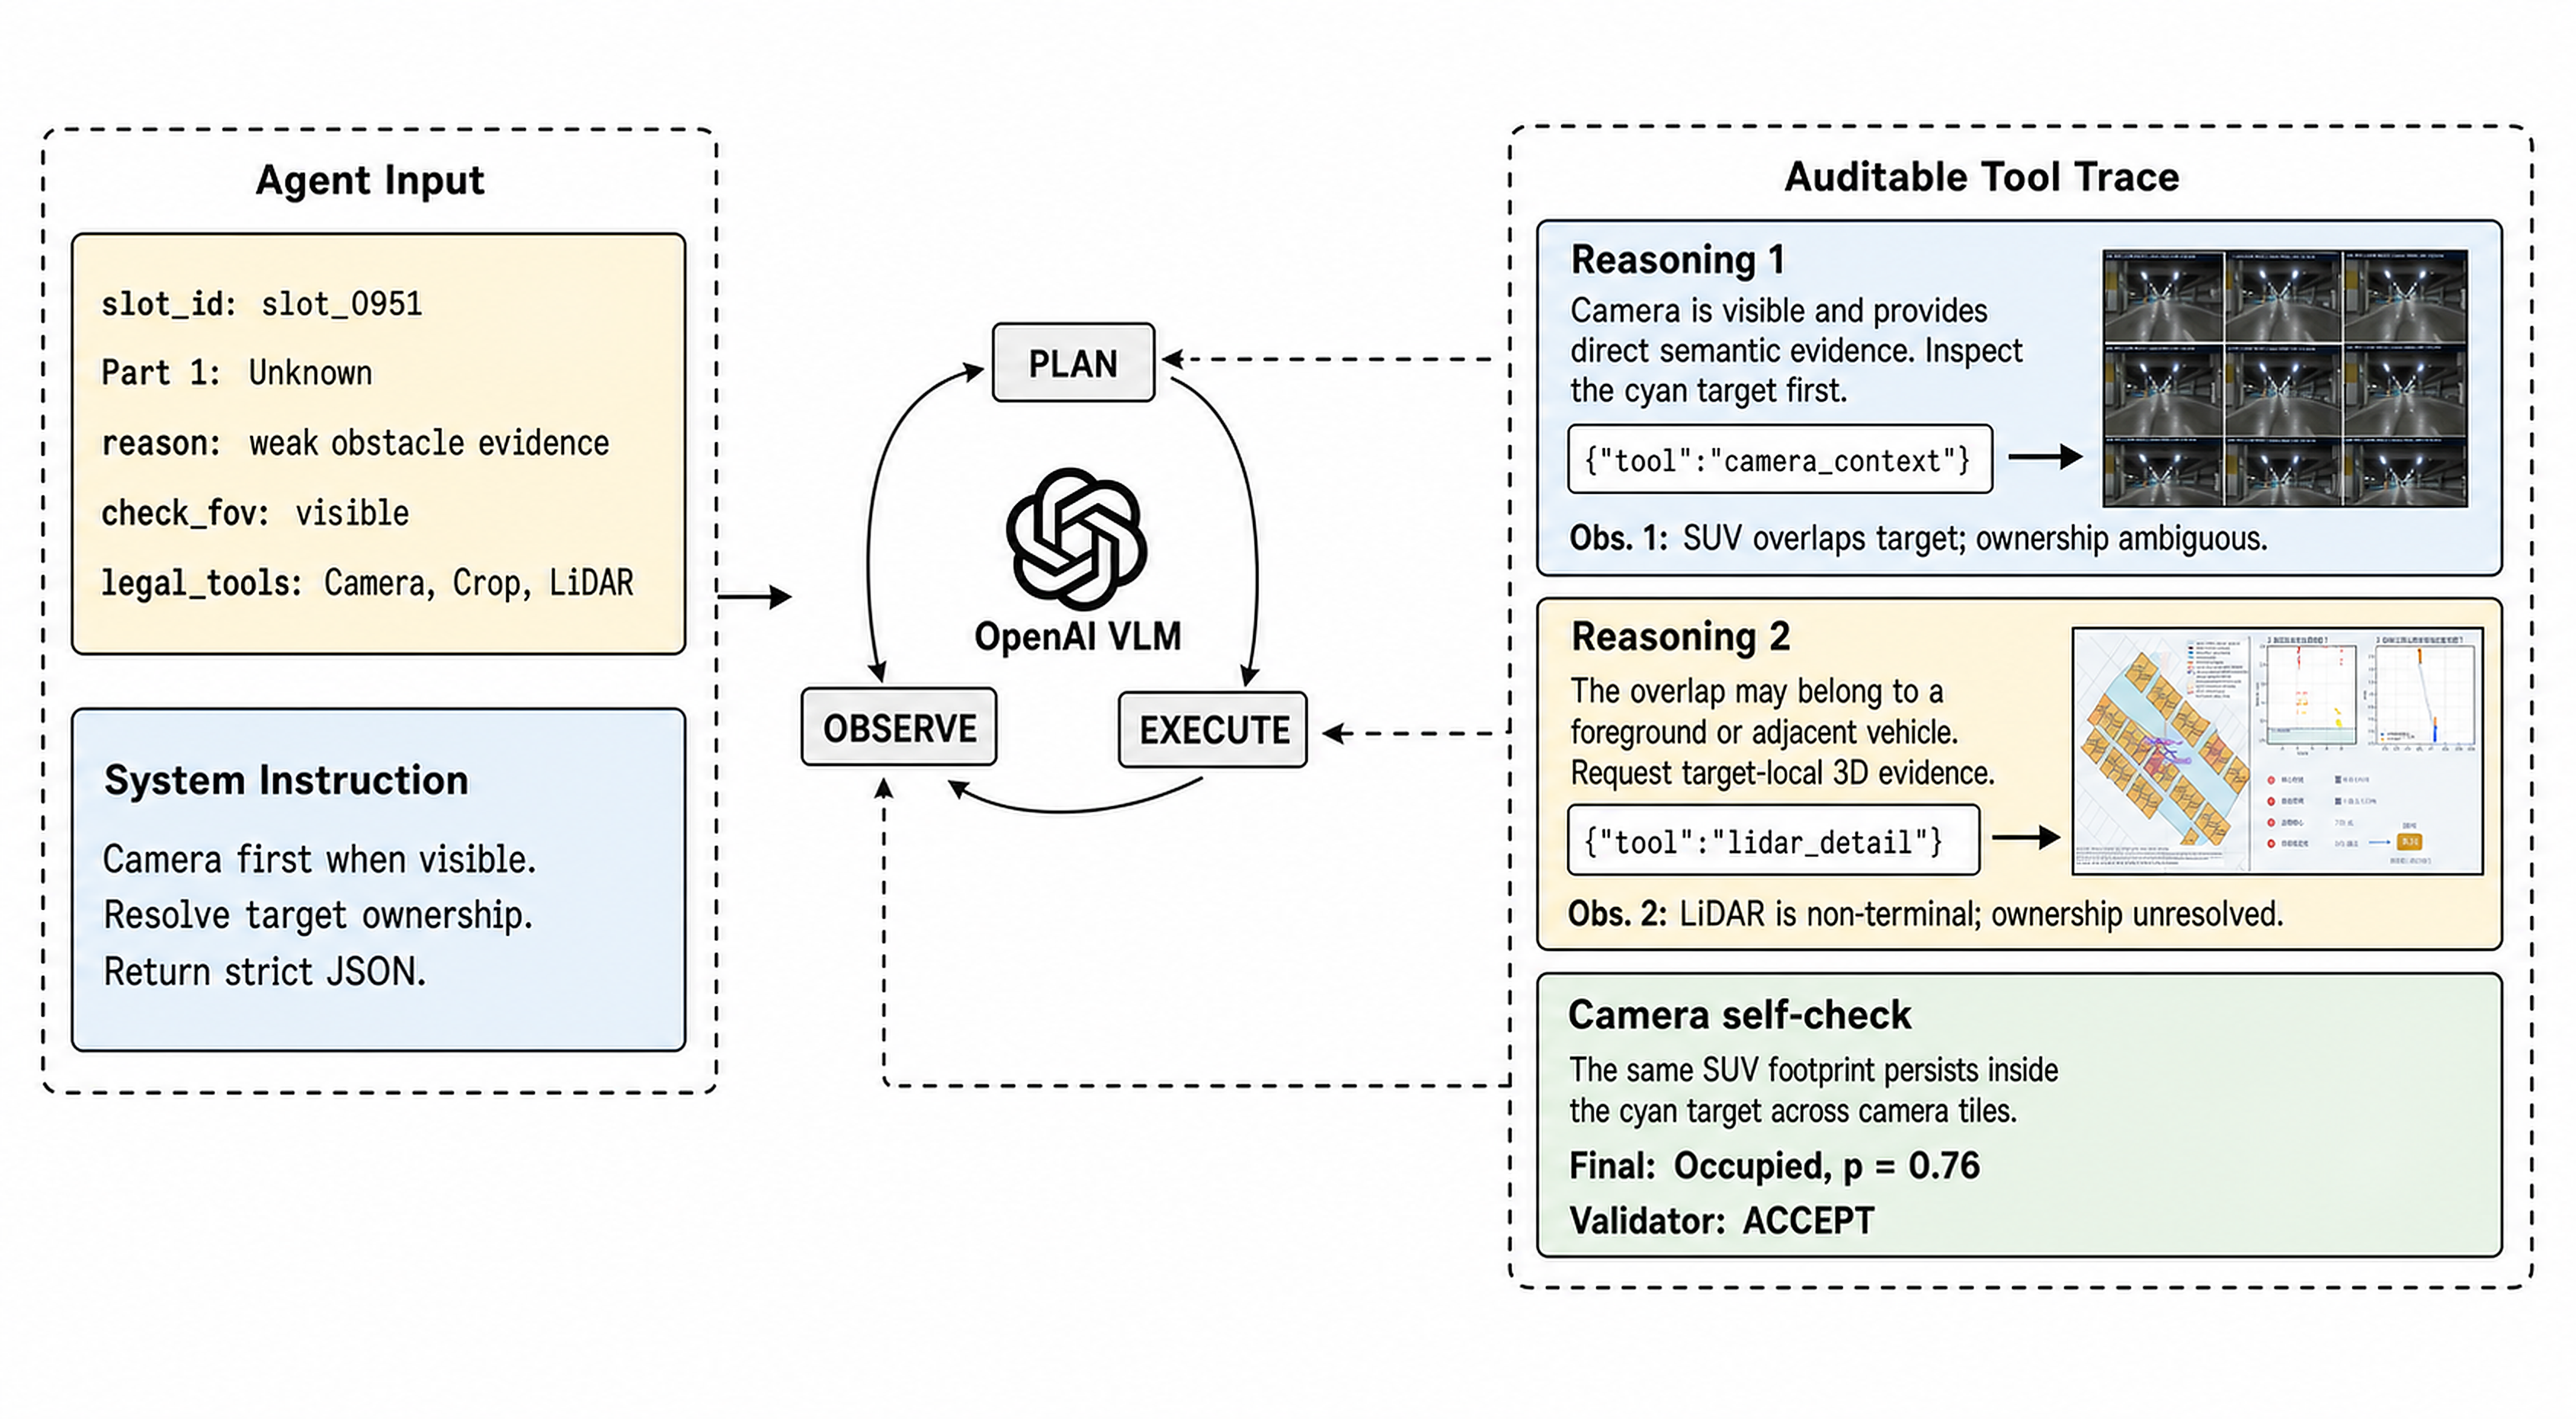
\includegraphics[width=0.99\textwidth]{figures/fig2_active_perception_trace_gptimage.png}
  \caption{Active perception in Part 2 for \texttt{slot\_0951}. The OpenAI center VLM receives a structured SlotCase and legal tool set, emits one JSON action per turn, observes the resulting evidence, and updates its belief. The displayed text is the persisted auditable reasoning summary, not hidden chain-of-thought. A deterministic validator rejects a non-terminal proposal and accepts the final evidence-bound Occupied decision at $p=0.76$.}
  \label{fig:active-agent}
\end{figure*}

\subsection{Evidence-Gated Terminal Decision}
The VLM proposal is not the system output. A terminal decision is accepted only when all cited evidence IDs have been observed, the predicted class satisfies modality-specific rules, and its required confidence is at least $\tau=0.60$. Camera-only Free or Occupied requires supported target localization and occupancy confidence. Occupied proposals made before a successful Part 2 detail observation are rejected. LiDAR can establish Free only through eligible clear-space geometry; obstacle returns alone cannot upgrade a visually ambiguous target to Occupied. If validation fails, the runtime requests a bounded correction or returns Unknown at the turn limit.

Formally, the validator separates a model proposal from an admissible system state:
\begin{equation}
\begin{aligned}
V_i={}&\mathbb{1}[\mathcal{E}^{\mathrm{cite}}_i
                   \subseteq\mathcal{E}^{\mathrm{obs}}_i]\\
     &\times\mathbb{1}[g_{\mathrm{mod}}(\hat y_i,
                    \mathcal{E}^{\mathrm{obs}}_i)=1]
       \mathbb{1}[p(\hat y_i)\geq\tau].
\end{aligned}
\end{equation}
The proposal is committed only when $V_i=1$; otherwise the validation error is returned to the agent while legal tools and turns remain, and the fail-closed terminal state is Unknown.

This architecture deliberately separates \emph{autonomy} from \emph{authority}. The VLM autonomously chooses which available observation to acquire and how to interpret it. The deterministic layer retains authority over which state transitions are admissible. Every completed run stores actions, observations, evidence bindings, validation errors, and a replay trace.


\begin{figure*}[t]
  \centering
  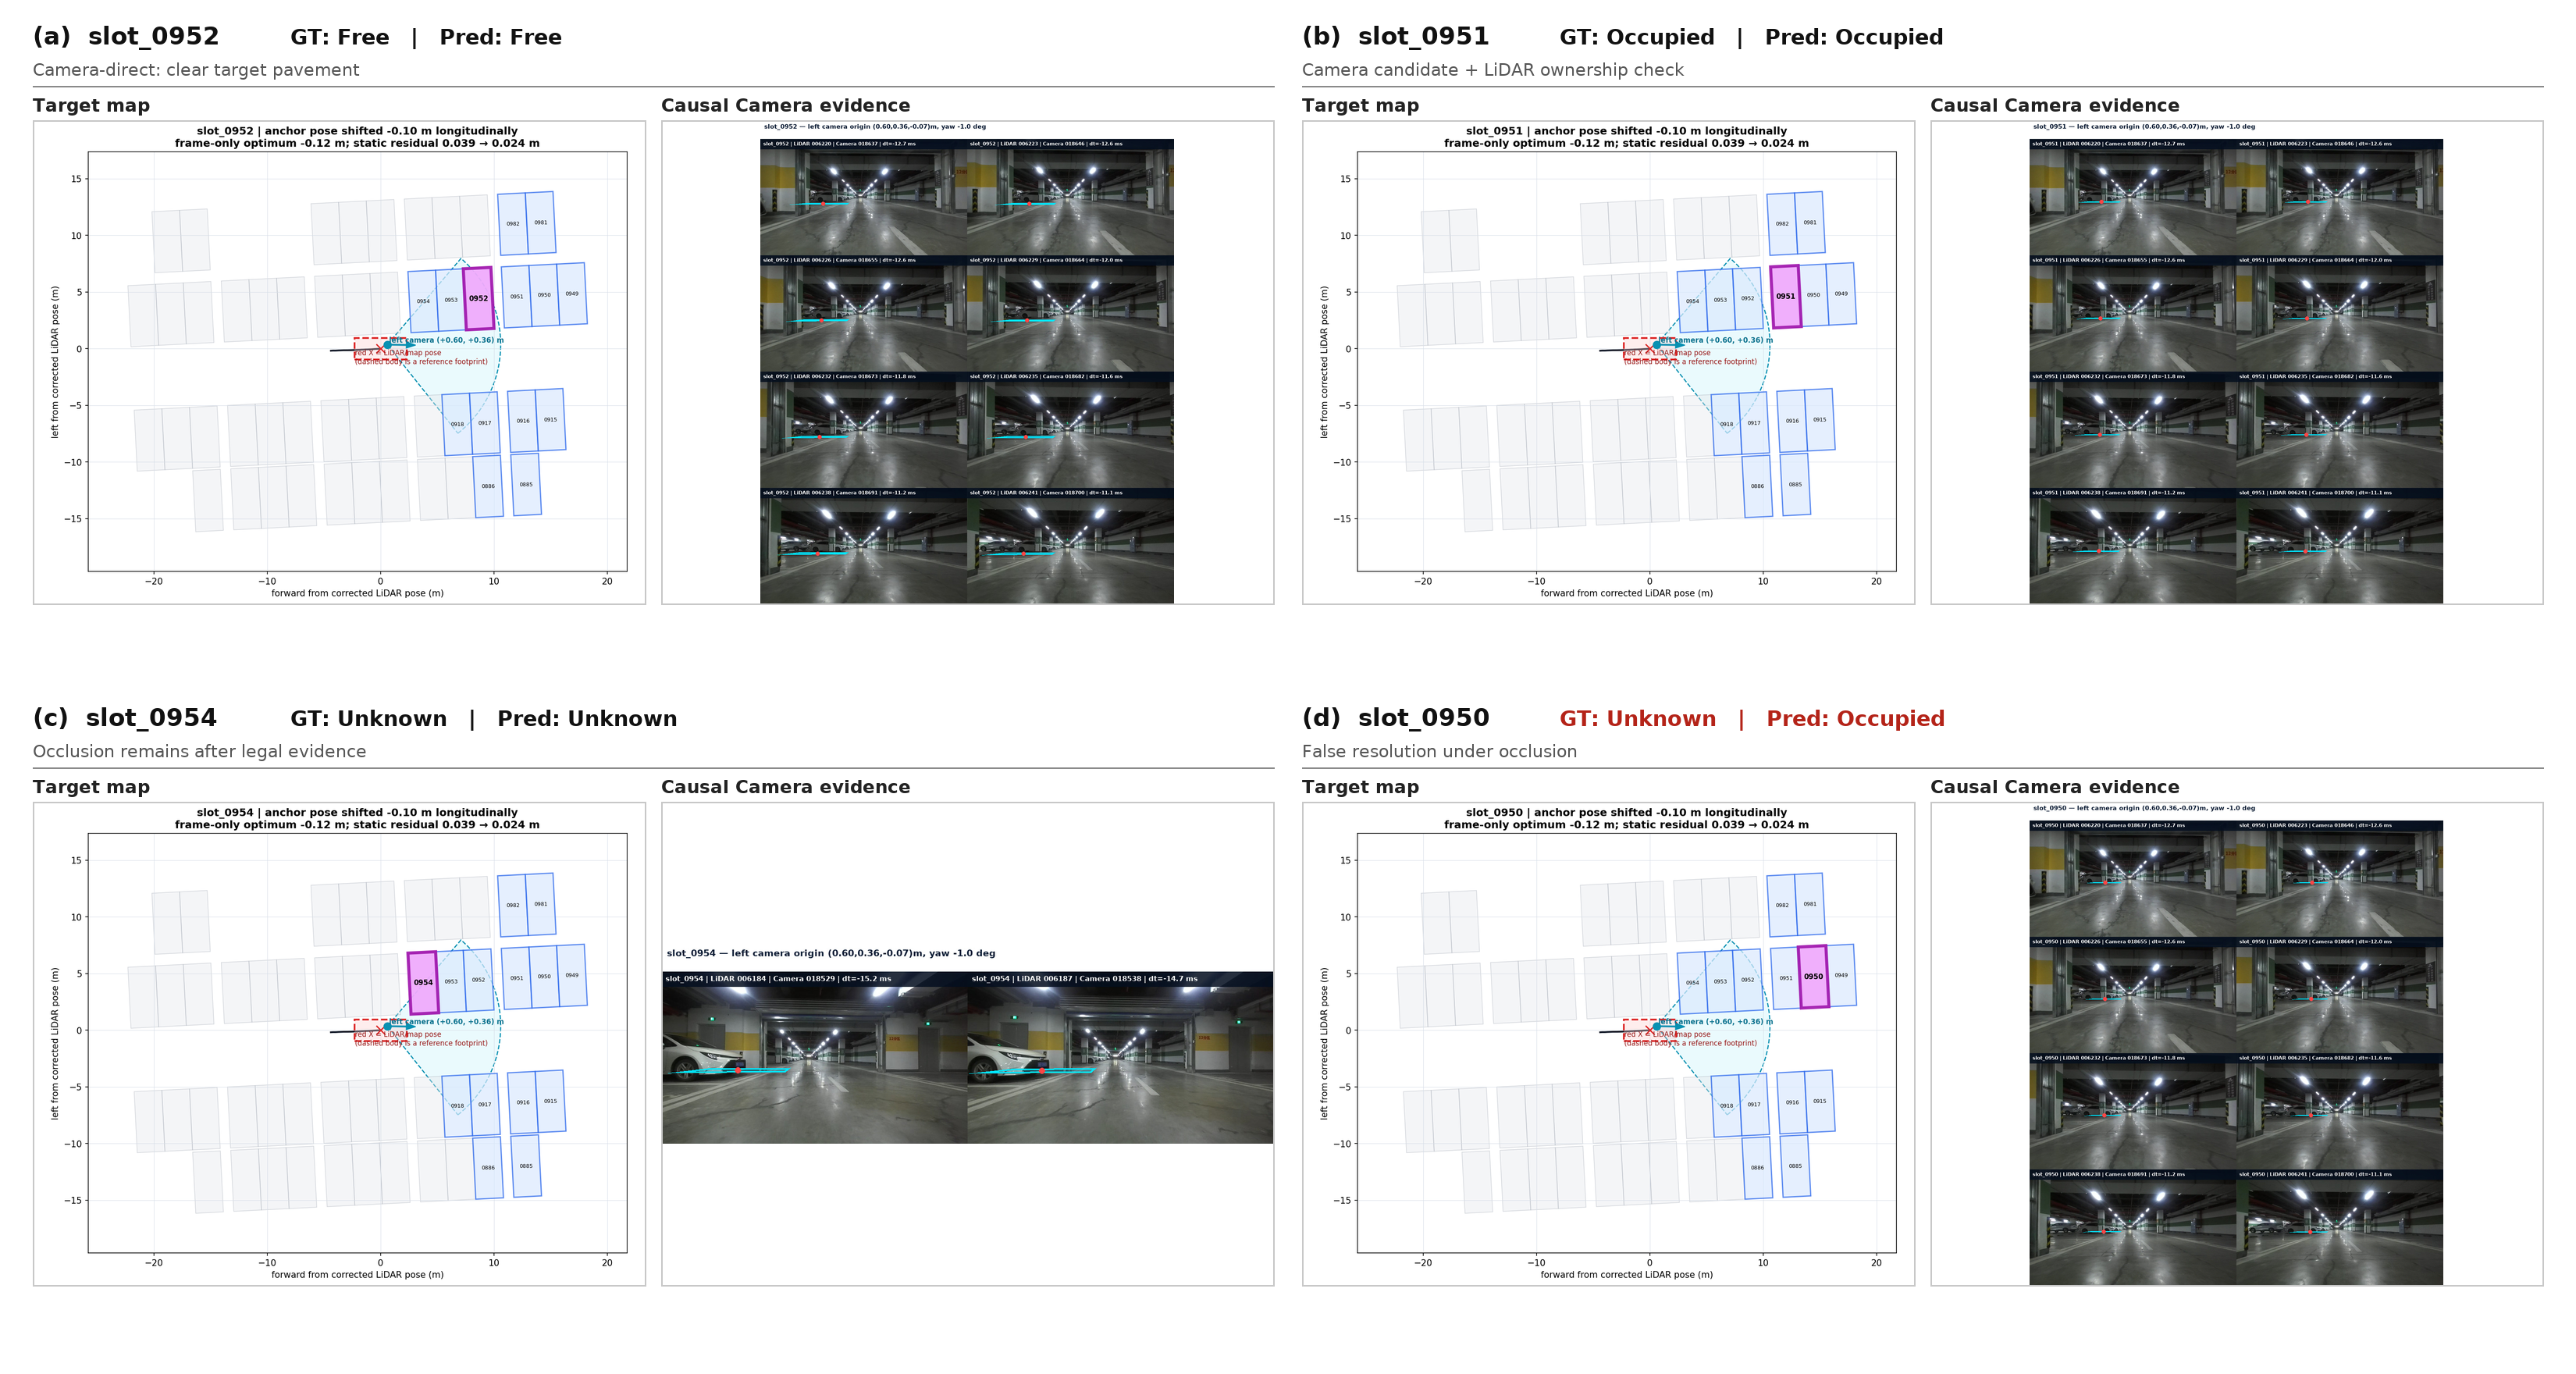
\includegraphics[width=0.98\textwidth]{figures/fig3_multicase_evidence.png}
  \caption{Representative locked-GT cases. The comparison includes a Camera-direct Free decision, a Camera-plus-LiDAR Occupied decision, correct abstention under occlusion, and the sole false resolution of a human-Unknown bay. Each column pairs the target map with its causal Camera evidence.}
  \label{fig:qualitative}
\end{figure*}

\section{Experiments}
\subsection{Experimental Protocol}
We evaluate on an instrumented parking-route sequence containing synchronized LiDAR, a left-facing camera, corrected map-frame poses, and a database of 1,397 mapped parking bays. The primary decision anchor is LiDAR frame 6241, associated with camera frame 18700. Local perception is restricted to 18~m and all historical inputs are causal.

The locked human annotation set contains 14 target bays: 6 Free, 2 Occupied, and 6 Unknown. Unknown includes genuinely occluded or identity-ambiguous cases rather than missing labels. Eleven unresolved, forward-facing bays are processed by Part 2; the remaining three retain their Part 1 output. The Part 2 input contains slot geometry, Part 1 evidence, unresolved reason codes, and tool resources, but not the human state.

We report (i) three-class accuracy over all 14 locked targets, (ii) terminal coverage, the fraction predicted Free or Occupied, (iii) terminal selective accuracy, accuracy conditioned on a terminal prediction, (iv) accuracy on the 11 Agent-processed cases, and (v) accuracy on the three human-marked camera-visible cases. Because the sample is small and comes from one anchor, all results are developmental rather than claims of route-level generalization.

\subsection{Main Results}
Table~\ref{tab:main} compares the selected Part 1 configuration with the complete camera-first system. Part 1 is intentionally conservative: it produces 13 Unknown predictions and one correct Occupied prediction, yielding 50.0\% three-class accuracy but 100\% selective accuracy at only 7.14\% coverage. The complete system resolves six Free bays and one additional Occupied bay correctly. It reaches 92.86\% overall accuracy, 64.29\% terminal coverage, and 88.89\% terminal selective accuracy. All eight determinate human labels are correct. The sole error is an Occupied prediction on a bay labeled Unknown, not a false Free.

The three camera-visible targets comprise two Free bays (\texttt{slot\_0952}, \texttt{slot\_0917}) and one Occupied bay (\texttt{slot\_0951}). All three are correct. This subset is defined by human observability, not merely by geometric field of view. A bay may project inside the camera and still be visually occluded.

\begin{table}[t]
\centering
\caption{Locked-GT results at frame 6241. Best values are bold. False-U is the percentage of human-Unknown bays incorrectly resolved to a terminal state.}
\label{tab:main}
\footnotesize
\resizebox{\columnwidth}{!}{%
\begin{tabular}{lcccccc}
\toprule
Method & Acc.$\uparrow$ & Cov.$\uparrow$ & Sel. Acc.$\uparrow$ & Agent-11$\uparrow$ & Visible-3$\uparrow$ & False-U$\downarrow$ \\
\midrule
\multicolumn{7}{c}{\textit{Geometry-only inference}} \\
Part 1, $W45/K3$ & 50.00 & 7.14 & \textbf{100.00} & -- & -- & \textbf{0.00} \\
\midrule
\multicolumn{7}{c}{\textit{Decision-aware active perception}} \\
DASP-Park full & \textbf{92.86} & \textbf{64.29} & 88.89 & \textbf{90.91} & \textbf{100.00} & 16.67 \\
\bottomrule
\end{tabular}
}
\end{table}

Figure~\ref{fig:qualitative} compares four qualitatively distinct outcomes. For \texttt{slot\_0952}, repeated clear target pavement supports a Camera-direct Free decision. For \texttt{slot\_0951}, the apparent target-owned vehicle is first identified in Camera and then checked with target-local LiDAR before Occupied is accepted. \texttt{slot\_0954} remains Unknown because occlusion survives all legal observations, demonstrating correct abstention. Finally, \texttt{slot\_0950} exposes the principal failure mode: a human-Unknown target is falsely resolved as Occupied under occlusion. Reporting this negative case prevents the aggregate 92.86\% accuracy from hiding the system's remaining ownership error.

\subsection{Runtime Audit}
The full run processes all 11 candidates and invokes camera context first in 11/11 cases. Ten cases subsequently use target-local LiDAR. Replay reproduces the complete semantic result. The reported accuracy is computed only after inference by joining predictions to locked slot identifiers. This separation is important: it prevents human labels from acting as model hints and permits independent inspection of every accepted or rejected action.

\section{Ablation Study}
\subsection{Temporal History Span and Sampling}
We evaluate 16 combinations with $W\in\{15,30,45,60\}$ and $K\in\{3,5,10,15\}$. Candidate identities and the current GT are fixed. The selection criterion first maximizes terminal selective accuracy, then minimizes false resolution of Unknown, and only then considers overall accuracy, coverage, and evidence cost.

Table~\ref{tab:history} shows the complete revised-GT sweep. $W45/K3$ and $W60/K5$ are the only configurations achieving 100\% terminal selective accuracy with zero false resolution of Unknown. We select $W45/K3$ because it uses the shorter span and fewer frames. Increasing $K$ is not monotonically beneficial: $W60/K10$ and $W60/K15$ increase terminal coverage to 14.29\% but reduce accuracy to 28.57\% and falsely resolve 33.33\% of Unknown targets. More history can accumulate misregistration and static-boundary contamination as well as useful evidence.

\begin{table}[t]
\centering
\caption{Complete Part 1 history ablation under the revised GT. Values are percentages; bold denotes the selected setting and underline denotes the runner-up under the safety-first ranking.}
\label{tab:history}
\scriptsize
\resizebox{\columnwidth}{!}{%
\begin{tabular}{ccrrrr}
\toprule
$W$ & $K$ & Acc.$\uparrow$ & Cov.$\uparrow$ & Sel. Acc.$\uparrow$ & False-U$\downarrow$ \\
\midrule
\multirow{4}{*}{15} & 3  & 42.86 & 14.29 & 50.00 & 16.67 \\
                    & 5  & 42.86 & 14.29 & 50.00 & 16.67 \\
                    & 10 & 42.86 & 14.29 & 50.00 & 16.67 \\
                    & 15 & 42.86 & 14.29 & 50.00 & 16.67 \\
\midrule
\multirow{4}{*}{30} & 3  & 42.86 & 0.00  & --    & 0.00 \\
                    & 5  & 35.71 & 7.14  & 0.00  & 16.67 \\
                    & 10 & 35.71 & 7.14  & 0.00  & 16.67 \\
                    & 15 & 35.71 & 7.14  & 0.00  & 16.67 \\
\midrule
\multirow{4}{*}{45} & \textbf{3}  & \textbf{50.00} & \textbf{7.14} & \textbf{100.00} & \textbf{0.00} \\
                    & 5  & 42.86 & 14.29 & 50.00 & 16.67 \\
                    & 10 & 35.71 & 7.14  & 0.00  & 16.67 \\
                    & 15 & 35.71 & 7.14  & 0.00  & 16.67 \\
\midrule
\multirow{4}{*}{60} & 3  & 42.86 & 0.00  & -- & 0.00 \\
                    & \underline{5}  & \underline{50.00} & \underline{7.14} & \underline{100.00} & \underline{0.00} \\
                    & 10 & 28.57 & 14.29 & 0.00 & 33.33 \\
                    & 15 & 28.57 & 14.29 & 0.00 & 33.33 \\
\bottomrule
\end{tabular}
}
\end{table}

\begin{figure*}[t]
  \centering
  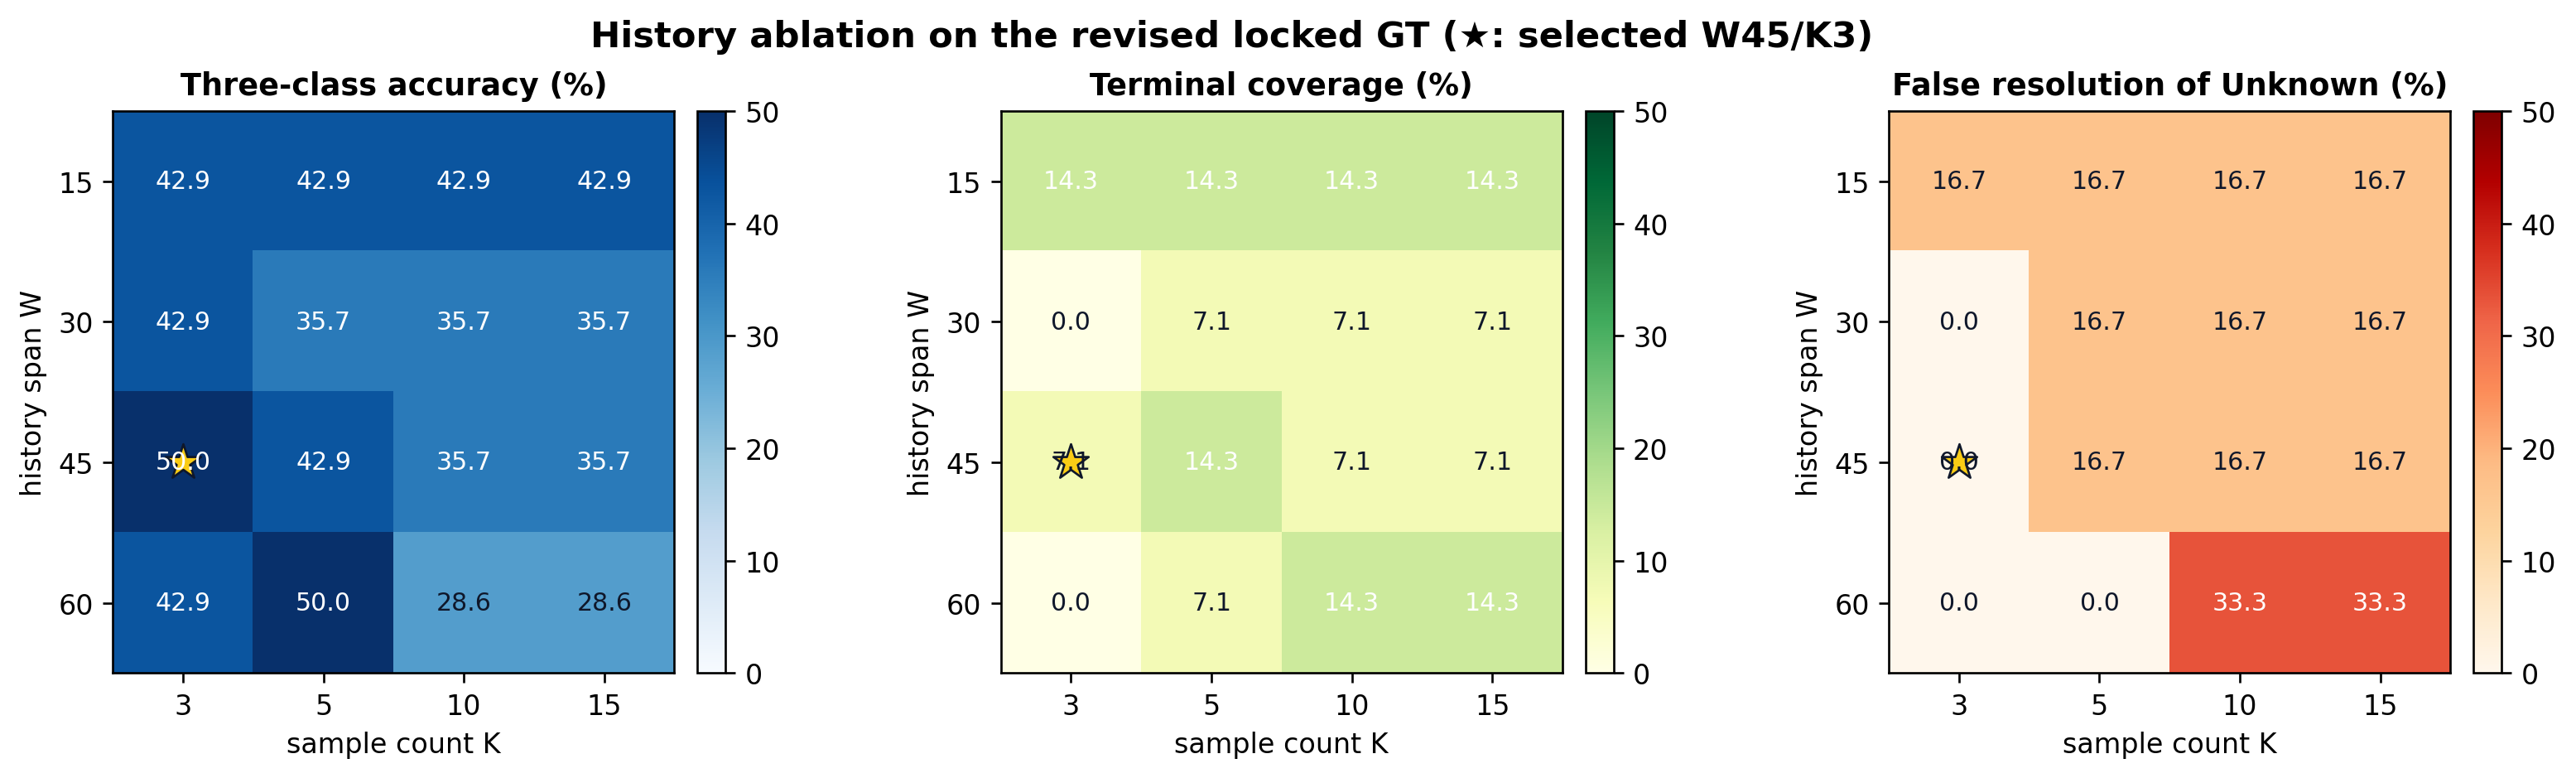
\includegraphics[width=0.94\textwidth]{figures/fig3_history_ablation.png}
  \caption{Temporal-history ablation over all 16 $(W,K)$ settings. The three heatmaps report overall three-class accuracy, terminal coverage, and false resolution of human-Unknown bays. The star marks the selected safety-first operating point $W{=}45,K{=}3$.}
  \label{fig:history-ablation}
\end{figure*}

\subsection{Center-VLM Capacity}
We self-deploy Qwen3-VL-2B-Instruct~\cite{qwen3vl2025} and Qwen3.5-0.8B~\cite{qwen35model2026} on the same RTX 5090. The 0.8B model is the closest official model to the requested ``0.7B class.'' The controlled pair uses byte-identical prompts, the same strict action JSON schema, the same 11 cases, identical tools, a six-turn limit, and $\tau=0.60$. Only model weights change. The previously completed OpenAI run is shown as contextual reference, not a strict member of this capacity ablation, because its frozen prompt predates the later camera-crop instructions.

Table~\ref{tab:vlm} reveals a protocol-level capacity gap. The 2B model correctly calls camera context first for all 11 candidates and reads images on 48 of 59 valid model actions. It then proposes 46 camera crops without satisfying the localization contract, so those executions are rejected; two Camera-based Free proposals also fail the terminal localization/occupancy gate. The 0.8B model never calls a detail tool. Its 60 valid structured actions are all direct finals---45 Occupied, 12 Free, and 3 Unknown---with zero input images. The runtime rejects these unsupported proposals and safely returns Unknown.

Both local models therefore reproduce the Part 1 system result after merging: 50.0\% accuracy, 7.14\% coverage, and 0\% camera-visible accuracy. This equality in final metrics masks a substantial behavioral difference. The 2B model understands camera-first planning but fails a finer localization protocol; the 0.8B model fails before evidence acquisition. Lowering the final confidence threshold would not address either failure and would admit evidence-free labels.

\begin{table}[t]
\centering
\caption{Center-VLM ablation. OpenAI is contextual only; the two self-deployed rows form the strict model-only comparison.}
\label{tab:vlm}
\footnotesize
\resizebox{\columnwidth}{!}{%
\begin{tabular}{lcccccc}
\toprule
Center model & Params & 14-GT$\uparrow$ & Agent-11$\uparrow$ & Visible$\uparrow$ & First Cam.$\uparrow$ & Replay \\
\midrule
\multicolumn{7}{c}{\textit{Cloud reference (not capacity-controlled)}} \\
OpenAI reference & -- & 92.86 & 90.91 & 100.0 & 11/11 & yes \\
\midrule
\multicolumn{7}{c}{\textit{Self-deployed, identical prompt/tools/runtime}} \\
Qwen3-VL & 2B & \textbf{50.00} & \textbf{36.36} & \textbf{0.0} & \textbf{11/11} & yes \\
Qwen3.5 & 0.8B & \textbf{50.00} & \textbf{36.36} & \textbf{0.0} & 0/11 & yes \\
\bottomrule
\end{tabular}
}
\end{table}

\begin{figure}[t]
  \centering
  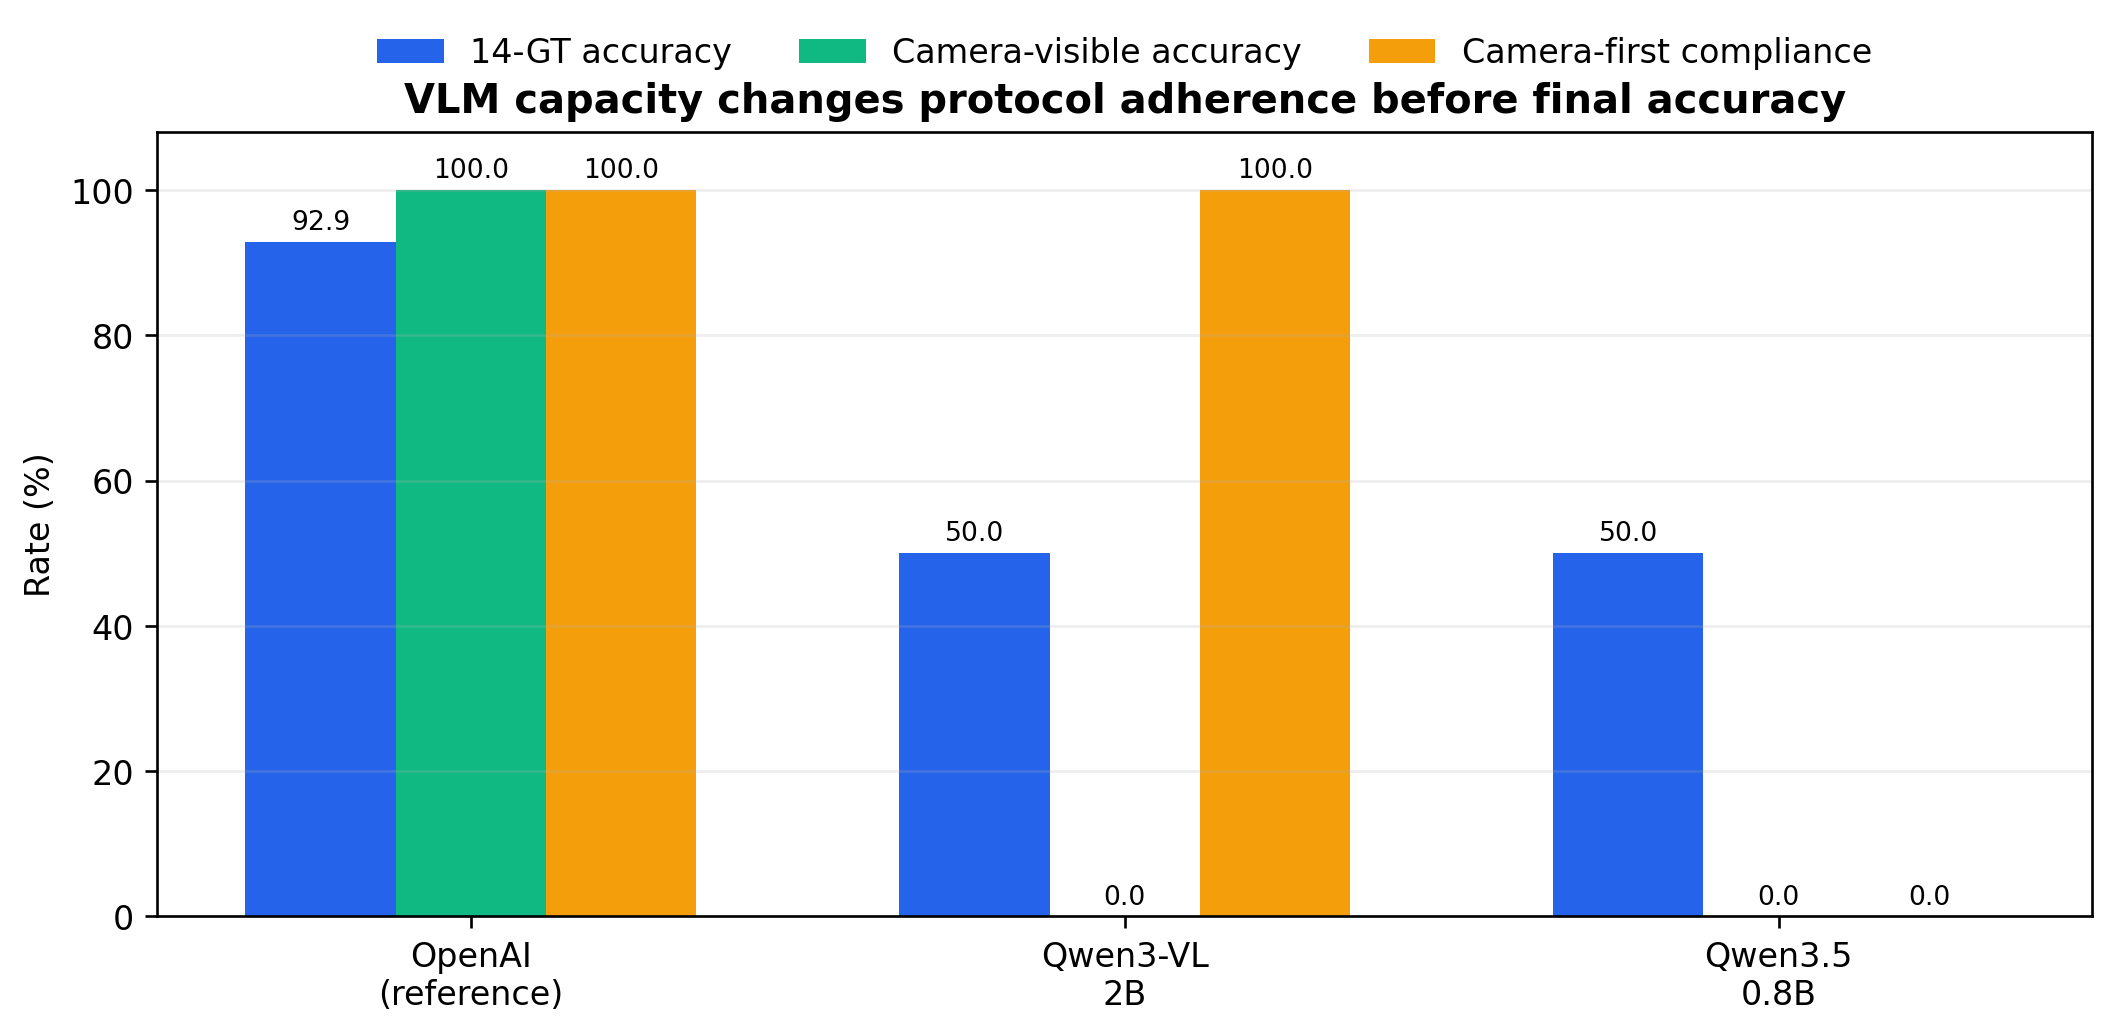
\includegraphics[width=0.98\columnwidth]{figures/fig4_vlm_ablation.png}
  \caption{Center-VLM comparison. Accuracy alone hides a protocol gap: Qwen3-VL-2B enters the camera-first tool loop, whereas Qwen3.5-0.8B produces unsupported direct labels and is rejected by the validator. OpenAI is shown as contextual reference.}
  \label{fig:vlm-ablation}
\end{figure}

\section{Discussion and Conclusion}
DASP-Park demonstrates that parking-slot occupancy benefits from separating evidence acquisition, semantic reasoning, and terminal authority. The geometric stage prevents absence of points from being mistaken for free space and prevents compact static structures from being mistaken for vehicles. The agent stage adds visual interpretation and can choose incremental evidence rather than applying a fixed fusion rule. The validator ensures that model fluency does not substitute for observation.

The results also clarify the role of Unknown. Part 1's 100\% selective accuracy is obtained at very low coverage; this is safe but not operationally sufficient. The camera-first agent increases coverage by 57.15 percentage points while preserving all determinate labels, but it makes one unsupported terminal resolution on a human-Unknown bay. Thus, higher coverage must be evaluated jointly with false resolution of Unknown. The local-VLM study provides a second example: fail-closed validation makes both small models appear equally conservative, although their internal behavior differs dramatically. Agent evaluation should therefore include protocol adherence and tool traces, not only final labels.

Our study has important limitations. The locked GT contains only 14 bays from a single decision anchor, the camera-visible subset contains only three examples, and the prompt and operating point were developed on the same route context. The human labels are single-annotator adjudications rather than a multi-rater benchmark. The OpenAI reference and the strict Qwen pair use slightly different prompt versions, so no direct capacity-only claim is made across those families. Finally, the method assumes a pre-existing slot map and corrected poses; robustness to cross-parking-lot map error remains unmeasured.

Future evaluation should freeze the full method before collecting a route-disjoint, multi-annotator dataset stratified by visibility, static structure, and occupancy. Confidence intervals should be clustered by route or anchor, and risk--coverage curves should accompany accuracy. Additional ablations should isolate camera context, crop, target-local LiDAR, pose uncertainty, and each class of deterministic validator. Larger local VLMs and schema-aware fine-tuning are promising because the 2B result suggests that tool acquisition emerges before reliable contract compliance.

In conclusion, DASP-Park offers a practical architecture for reliable parking-slot reasoning under occlusion: temporal geometry proposes what is known, a multimodal agent decides what to inspect, and an evidence validator decides what may become certain. The developmental results are encouraging, but the strongest finding is methodological rather than numerical: autonomous perception agents should be free to seek evidence and required to prove that they used it.

\balance
\bibliographystyle{IEEEtran}
\bibliography{references}
\end{document}
